\section{Całkowanie metodą ,,orzeł-reszka''}
%%%%%%%%%%%%%%%%
\begin{frame}{Całkowanie metodą ,,orzeł-reszka''}
	Szukamy $I = \int_0^1 f(x) dx; 0 \le f(x) \le 1$
    
    {\centering 
    	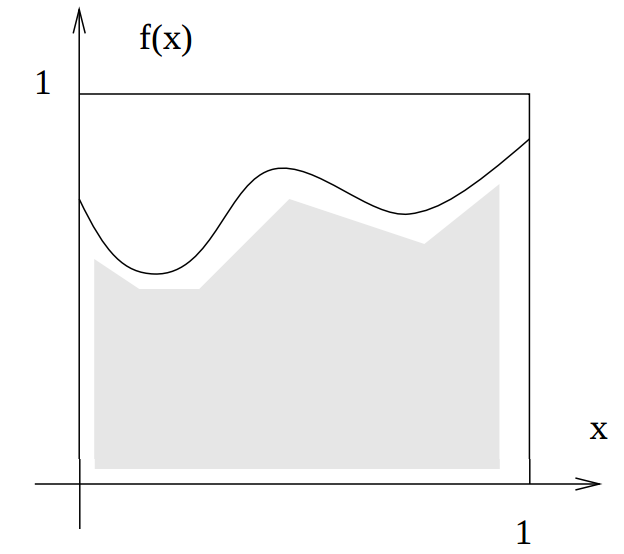
\includegraphics[width=.4\linewidth]{img/15/15_1_orzel_reszka}
        \par
    }
    
    $(X, Y)$ - dwuwymiarowa zmienna losowa o rozkładzie równomiernym na kwadracie: $(0 \le x \le 1, 0 \le y \le 1)$ \\
    Prawdopodobieństwo, że $(X, Y)$ przyjmie wartość z zakreskowanej części rysunku jest równe tej powierzchni, czyli wartości całki $I$.
\end{frame}
%%%%%%%%%%%%%%%%
\begin{frame}{Metoda}
	$N$ - eksperymentów: obserwacji $(X, Y)$ \\
    $M$ - liczba eksperymentów, w których $(X, Y)$ poniżej $f(x)$
    \\[8pt]
    Jeżeli obserwacje niezależne - to $M$ ma rozkład dwumianowy
    
    \[\boxed{
    	P\{M = m\} = \left(
            \frac{N}{m}
        \right) I^m (1-I)^{N-m}
    }\]
\end{frame}
%%%%%%%%%%%%%%%%
\begin{frame}{Metoda}
	Zadanie:\\
    oszacowanie $\hat{I} = \frac{M}{N}$ \\
    wariancja $S^2(\hat{I}) = \frac{1}{N} \frac{M}{N} \left( 
    	1 - \frac{M}{N}
    \right)$ 
    \\[8pt]
    Metoda:
    \begin{itemize}
    	\item prosta,
        \item łatwe uogólnienie na n-D
        \item mało efektywna
    \end{itemize}
\end{frame}